\chapter{DESENVOLVIMENTO}

\section{Diodo Ideal}

\begin{figure}[H]
    \centering
    \fbox{
        \parbox{0.975\textwidth}{
            \centering
            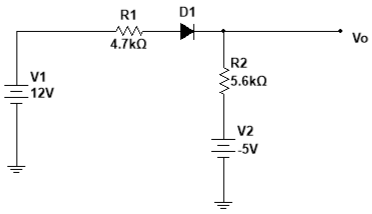
\includegraphics[width=0.975\textwidth]{images/Circuito01.png}
        }}
    \caption{Circuito 01}
    \vspace{-0.3cm}
    \label{fig:Circuito01}
\end{figure}

Encontre no circuito da imagem \ref{fig:Circuito01} IR1, VR1, VR2 e Vo.

\noindent
\textbf{Resolução}

\begin{Resolucao}[H]
    \fbox{
        \parbox{0.975\textwidth}{
            \vspace{0.40cm}
            \centering
            \[+12 - 4.7KI - 5.6KI - (-5) = 0\]
            \[IR1 = \frac{12-(-5)}{4.7K + 5.6K} = \textcolor{red}{1.65mA}\]
            \[\frac{5.6K}{4.7K + 5.6K} \simeq 0.54 * 12 = \textcolor{red}{6.52V}\]
            \[\frac{4.7K}{4.7K + 5.6K} \simeq 0.45 * 5 = \textcolor{red}{2.28V}\]
            \[Vo = 6.52 - 2.28 \simeq \textcolor{red}{4.24V}\]
        }
    }
    \captionof*{Resolucao}{Resolução: Circuito 01}
    \label{res:Circuito01}
\end{Resolucao}

\section{Diodo Linear}

\begin{figure}[H]
    \centering
    \fbox{
        \parbox{0.975\textwidth}{
            \centering
            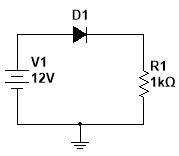
\includegraphics[]{images/Circuito02.png}
        }}
    \caption{Circuito 02}
    \vspace{-0.3cm}
    \label{fig:Circuito02}
\end{figure}

Analisando o circuito da imagem \ref{fig:Circuito01} com um diodo linear, substituiremos o diodo por uma fonte de tensão ideal de 0.7V seguido por um resistor de 10$\Omega$, conforme a imagem \ref{fig:Circuito03}.

\begin{figure}[H]
    \centering
    \fbox{
        \parbox{0.975\textwidth}{
            \centering
            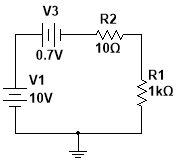
\includegraphics[]{images/Circuito03.png}
        }}
    \caption{Circuito 03}
    \vspace{-0.3cm}
    \label{fig:Circuito03}
\end{figure}

\begin{Resolucao}[H]
    \fbox{
        \parbox{0.975\textwidth}{
            \vspace{0.40cm}
            \centering
            \[It = \frac{10 - 0.7}{1K + 10} = \textcolor{red}{9.207mA} \]

        }
    }
    \captionof*{Resolucao}{Resolução: Circuito 02}
    \label{res:Circuito02}
\end{Resolucao}

Através da imagem \ref{fig:SimulacaoCircuito02} podemos verificar os resultados obtidos por simulação. 

\begin{figure}[H]
    \centering
    \fbox{
        \parbox{0.975\textwidth}{
            \centering
            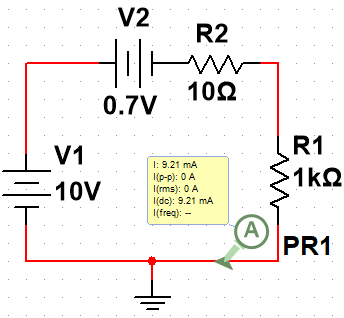
\includegraphics[]{images/simulacoes/circuito03.png}
        }}
    \caption{Simulação do circuito 02}
    \vspace{-0.3cm}
    \label{fig:SimulacaoCircuito02}
\end{figure}

Com a tabela \ref{tab:Comparacao1Circuito} podemos comparar os resultados obtidos por simulação com os resultados obtidos por cálculo, na qual comprovam que os cálculos estavam corretos, com uma pequena diferença devido a aproximação.

\begin{quadro}[H]
    \centering
    \caption{Comparação entre os resultados obtidos por simulação e os resultados obtidos por cálculo do circuito 02}
    \begin{tabular}{|C{0.34\textwidth}|C{0.19\textwidth}|C{0.19\textwidth}|C{0.19\textwidth}|C{0.19\textwidth}|}
        \hline
        \rowcolor[HTML]{C0C0C0}
        \textbf{Modelo\textbackslash{}Variáveis} & \textbf{It} \\
        \hline
        Calculado & 9.207mA \\
        \hline
        Simulado & 9.210mA \\
        \hline
    \end{tabular}
    \vspace{-0.6cm}
    \label{tab:Comparacao1Circuito}
\end{quadro}

\section{Diodo Real}

Para realizar a análise de um diodo real, é necessário obter a sua reta de carga, e utilizar as equações a seguir para obter 2 pontos através da reta de carga, para que assim possamos obter a reta de carga do circuito.

\noindent
\textbf{Equações}

\begin{Resolucao}[H]
    \fbox{
        \parbox{0.975\textwidth}{
            \vspace{0.40cm}
            \centering
            \[Id = \frac{-Vd + Vf}{RL}\]
            \[\textnormal{Se Vd = 0 $\rightarrow$ } Vd = \frac{Vf}{RL}\]
            \[\textnormal{Se Id = 0 $\rightarrow$ } Id = Vf\]
        }
    }
    \captionof*{Resolucao}{Equações: Reta de carga de diodo real}
    \label{res:Circuito02}
\end{Resolucao}

\subsection{Curva característica do diodo}

A imagem \ref{fig:Circuito04} mostra o circuito montado por simulação para se obter a curva característica do diodo 1N4007G, e a imagem \ref{fig:curva_diodo_polarizado} mostra a curva característica do diodo 1N4007G.

\begin{figure}[H]
    \centering
    \fbox{
        \parbox{0.975\textwidth}{
            \centering
            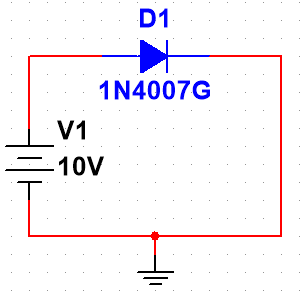
\includegraphics[]{images/simulacoes/circuito04.png}
        }}
    \caption{Simulação do circuito 03}
    \vspace{-0.3cm}
    \label{fig:Circuito04}
\end{figure}

\begin{figure}[H]
    \centering
    \fbox{
        \parbox{0.975\textwidth}{
            \centering
            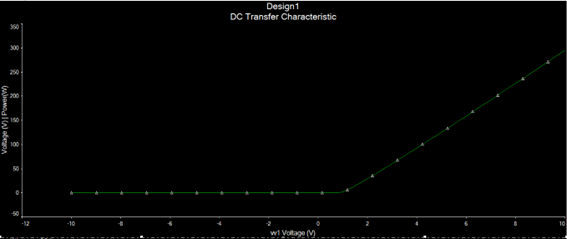
\includegraphics[]{images/curva_diodo_polarizado.png}
        }}
    \caption{Curva característica do diodo do circuito 03}
    \vspace{-0.3cm}
    \label{fig:curva_diodo_polarizado}
\end{figure}

Realizando uma análise sobre a reta de carga do diodo polarizado, é possível perceber que o diodo começa permitir a passagem de corrente ao chegar uma tensão de 0.7V, que é a tensão necessária para romper a barreira da tensão real do diodo.

\begin{figure}[H]
    \centering
    \fbox{
        \parbox{0.975\textwidth}{
            \centering
            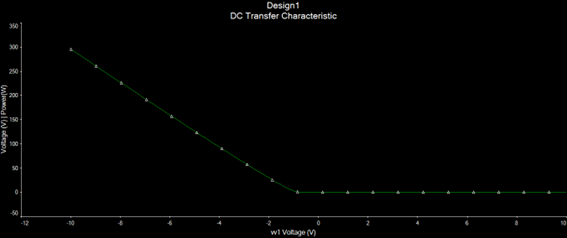
\includegraphics[]{images/curva_diodo_nao_polarizado.png}
        }}
    \caption{Curva característica do diodo do circuito 03 não polarizado}
    \vspace{-0.3cm}
    \label{fig:curva_diodo_nao_polarizado}
\end{figure}

Na imagem \ref{fig:curva_diodo_nao_polarizado}, podemos observar a reta de carga de um diodo polarizado de maneira reversa, onde se conclui que o mesmo conduz até se chegar em uma carga menor que 0.7, onde a tensão do diodo começa a ser maior que a tensão aplicada, e assim o diodo não consegue conduzir corrente.

Com estes conhecimentos prévios, análise o seguinte exercício da imagem \ref{fig:Circuito05}.

\begin{figure}[H]
    \centering
    \fbox{
        \parbox{0.975\textwidth}{
            \centering
            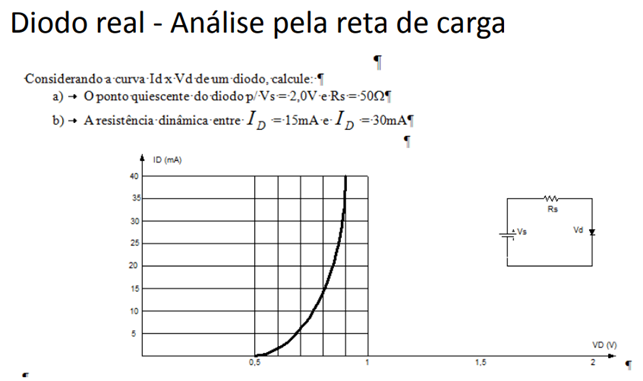
\includegraphics[]{images/exercicio_analise.png}
        }}
    \caption{Exercício - Reta de carga}
    \vspace{-0.3cm}
    \label{fig:Circuito05}
\end{figure}

\begin{figure}[H]
    \centering
    \fbox{
        \parbox{0.975\textwidth}{
            \centering
            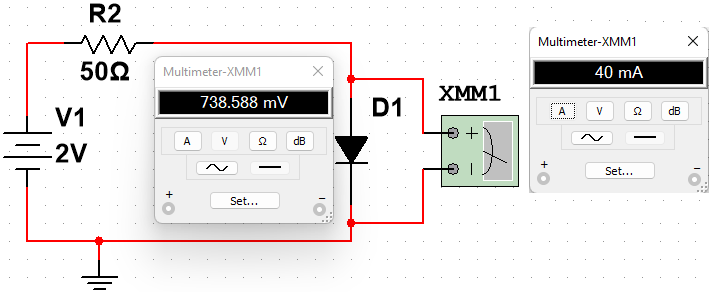
\includegraphics[width=0.975\textwidth]{images/simulacoes/circuito05.png}
        }}
    \caption{Simulação do exercício}
    \vspace{-0.3cm}
    \label{fig:SimulacaoCircuito05}
\end{figure}

\begin{figure}[H]
    \centering
    \fbox{
        \parbox{0.975\textwidth}{
            \centering
            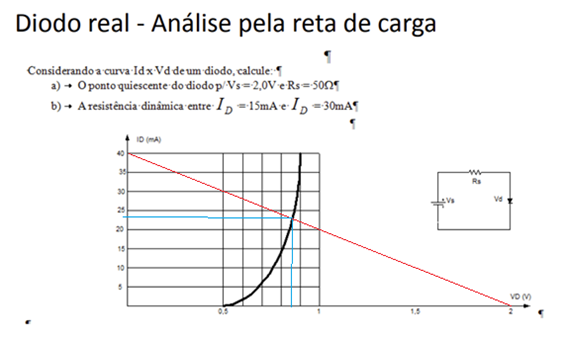
\includegraphics[width=0.975\textwidth]{images/analise_tracado.png}
        }}
    \caption{Traçado da reta de carga do exercício}
    \vspace{-0.3cm}
    \label{fig:TracadoRetaDeCarga}
\end{figure}

\noindent
\textbf{Resolução - A}

\begin{Resolucao}[H]
    \fbox{
        \parbox{0.975\textwidth}{
            \vspace{0.40cm}
            \centering
            Para VD = 0...
            \[Vf = Vd + Id * R\]
            \[2V = 0 + Id * 50\]
            \[Id = \frac{2V}{50} = \textcolor{red}{40mA}\]	

            Para Id = 0...
            \[Vd = Vs\]
            \[Vd = \textcolor{red}{2V}\]

            Após traçar a reta de carga (Imagem \ref{fig:TracadoRetaDeCarga})
            \[Vd \simeq \textcolor{red}{0.85V} \]
            \[Id \simeq \textcolor{red}{25mA}\]
        }
    }
    \captionof*{Resolucao}{Resolução: Circuito Exercício}
    \label{res:CircuitoExercicio}
\end{Resolucao}

\begin{figure}[H]
    \centering
    \fbox{
        \parbox{0.975\textwidth}{
            \centering
            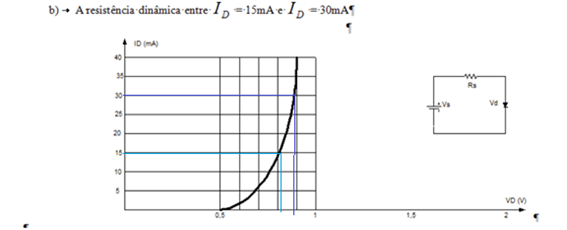
\includegraphics[width=0.975\textwidth]{images/analise_tracado2.png}
        }}
    \caption{Traçado da reta de carga do exercício B}
    \vspace{-0.3cm}
    \label{fig:TracadoRetaDeCargaB}
\end{figure}

\noindent
\textbf{Resolução - B}

\begin{Resolucao}[H]
    \fbox{
        \parbox{0.975\textwidth}{
            \vspace{0.40cm}
            \centering
            \[Id = 15mA \rightarrow \textcolor{red}{0.82V}\]
            \[Id = 30mA \rightarrow \textcolor{red}{0.88V}\]

            \[Rd = \frac{0.88 - 0.82}{30-15}\]
            \[\frac{60mV}{15mV} = 4\Omega\]
        }
    }
    \captionof*{Resolucao}{Resolução: Circuito Exercício}
    \label{res:CircuitoExercicio}
\end{Resolucao}